\documentclass[a4paper,12pt]{article}
\usepackage[a4paper,top=1.3cm,bottom=2cm,left=1.5cm,right=1.5cm,marginparwidth=0.75cm]{geometry}
\usepackage{cmap}
\usepackage{mathtext}
\usepackage[T2A]{fontenc}
\usepackage[utf8]{inputenc}
\usepackage[english,russian]{babel}
\usepackage{siunitx}

\usepackage{graphicx}

\usepackage{wrapfig}
\usepackage{tabularx}
\usepackage{multirow}

\usepackage{hyperref}
\usepackage[rgb]{xcolor}
\hypersetup{
colorlinks=true,urlcolor=blue
}
\usepackage{amsmath,amsfonts,amssymb,amsthm,mathtools}
\usepackage{icomma}
\mathtoolsset{showonlyrefs=false}
\usepackage{euscript}
\usepackage{mathrsfs}
\DeclareMathOperator{\sgn}{\mathop{sgn}}
\newcommand*{\hm}[1]{#1\nobreak\discretionary{}
{\hbox{$\mathsurround=0pt #1$}}{}}

%%% Заголовок
\author{Макаров Лев Евгеньевич}
\title{Лабораторная работа №1.2.5

Изучение экспериментальных погрешностей на примере физического маятника
}
\date{\today}

\begin{document}

\begin{titlepage}
	\begin{center}
		{\large МОСКОВСКИЙ ФИЗИКО-ТЕХНИЧЕСКИЙ ИНСТИТУТ (НАЦИОНАЛЬНЫЙ ИССЛЕДОВАТЕЛЬСКИЙ УНИВЕРСИТЕТ)}
	\end{center}
	\begin{center}
		{\large Физтех-школа фотоники, электроники и молекулярной физики}
	\end{center}
	
	
	\vspace{4.5cm}
	{\huge
		\begin{center}
			{\bf Отчёт о выполнении лабораторной работы 1.2.5}\\
			Исследование вынужденной регулярной прецессии гироскопа
		\end{center}
	}
	\vspace{2cm}
	\begin{flushright}
		{\LARGE Автор:\\ Макаров Лев Евгеньевич \\
			\vspace{0.2cm}
			Б04-306}
	\end{flushright}
	\vspace{8cm}
	\begin{center}
		Долгопрудный 2023
	\end{center}
\end{titlepage}

\section{Введение}

\textbf{Цель работы:} 
\begin{enumerate}
	\item исследовать вынужденную прецессию гироскопа
	\item установить зависимость скорости вынужденной прецессии от величины момента сил, действующих на ось гироскопа
        \item определить скорость вращения ротора гироскопа и сравнить ее со скоростью, рассчитан- ной по скорости прецессии
\end{enumerate}

\textbf{В работе используются:} 
\begin{itemize}
    \item гироскоп в кардановом подвесе
    \item секундомер
    \item набор грузов
    \item отдельный ротор гироскопа
    \item цилиндр известной массы
    \item крутильный маятник
    \item штангенциркуль
    \item линейка
\end{itemize}
\medskip

\section{Теоретические сведения}

Уравнения движения твердого тела можно записать в виде:

\begin{equation}
    \frac{d \vec{P}}{dt} = \vec{F}
\end{equation}

\begin{equation}\label{L-general}
    \frac{d \vec{L}}{dt} = \vec{M}
\end{equation}

В данной работе рассматривается задача о вращении твердого тела вокруг вокруг неподвижной точки. Момент импульса в его главных осях $x$, $y$, $z$ равен:

\begin{equation}
    \vec{L} = \vec{i} I_{x} \omega_{x} + \vec{j} I_{y} \omega_{y} + \vec{k} I_{z} \omega_{z}
\end{equation}

Где $I_{x}$, $I_{y}$, $I_{z}$ -- главные моменты инерции, $\omega_{x}$, $\omega_{y}$, $\omega_{z}$ -- компоненты вектора угловой скорости $\vec{\omega}$. Для гироскопа, быстро вращающегося тела, справедливо:

\begin{equation}
    I_{z} \omega_{z} \gg I_{x} \omega_{x}, \space I_{y} \omega_{y}
\end{equation}

Из \eqref{L-general} следует, что приращение момента импульса определяется следующим образом:

\begin{equation}\label{delta-l-int}
    \Delta \vec{L} = \int \vec{M} dt
\end{equation}

Если момент внешних сил действет в течение короткого промежутка времени, то из \eqref{delta-l-int} следует:

\begin{equation}
    \left | \Delta \vec{L} \right | \ll \left | \vec{L} \right |
\end{equation}

Поэтому движение гироскопа становится крайне устойчиво после приведения его в быстрое вращение.

Для выяснения сил, необходимых для изменения направления его оси, рассмотрим маховик изображенный на рис. \ref{machovik}, вращающийся вокру оси $z$, перепенликулярной к плоскости маховика.

\begin{figure}[h!]
        \centering
	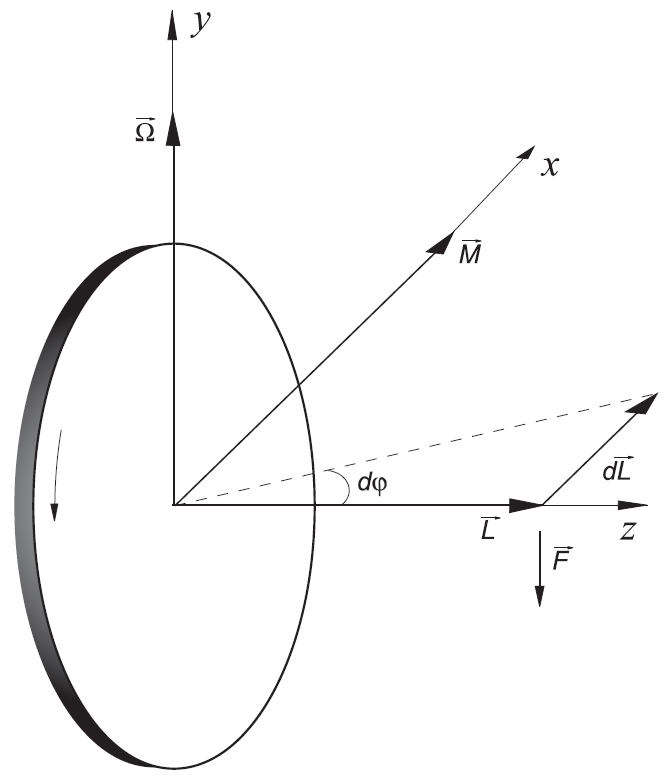
\includegraphics[width=0.3\textwidth]{mahovik.png}
	\caption{\textit{Маховик}}
	\label{machovik}
\end{figure}

Будем считать, что:

\begin{equation}
    \omega_{x} = \omega_{0}, \omega_{y} = 0, \omega_{z} = 0
\end{equation}

При повороте оси в плоскости $zx$ на малый угол $d \varphi$ появляется добавочное вращение маховика вокруг оси $y$, так что

\begin{equation}
    d \varphi = \Omega dt
\end{equation}

где угол $\Omega$ -- угловая скорость такого вращения. Будем считать, что

\begin{equation}\label{condition-9}
    L_{\Omega} \ll L_{\omega_{0}}
\end{equation}

Это означает, что момент импульса маховика, не изменяя своей величины, повернулся в плоскости $zx$. Таким образом:

\begin{equation}
    \left | d \vec{L} \right | = L d \varphi = L \Omega dt
\end{equation}

Вектор $d \vec{L}$ можно представить в виде векторного вроизведения угловой скорости $\vec{\Omega}$, направленного вдоль оси $y$, на вектор собственного момента импульса маховика, направленного вдоль оси $z$.

\begin{equation}
    d \vec{L} = \vec{\Omega} \times \vec{L} dt,
\end{equation}

\begin{equation}
    \frac{d \vec{L}}{dt} = \vec{\Omega} \times \vec{L}
\end{equation}

Это означает, что момент импульса вращается с постоянной угловой скоростью и неизменен по модулю. Из \eqref{L-general} имеем:

\begin{equation}\label{M-main}
    \vec{M} = \vec{\Omega} \times \vec{L}
\end{equation}

Формула \eqref{M-main} справедлива, если выполняется \eqref{condition-9}. Видно, что для поворота оси вращающегося маховика к оси $x$ необходимо приложить силы вдоль оси $y$, так чтобы их момент $\vec{M}$ был направлен вдоль оси $x$.

Под действием момента $\vec{M}$ внешних сил ось гироскопа медленно вращается вокруг оси $у$ с угловой скоростью $\Omega$. Такое движение назы- вается регулярной прецессией гироскопа. В частности, создающей мо мент внешней силой может оказаться сила тяжести, если центр масс гироскопа не совпадает с точкой подвеса. Для гироскопа массой $m_{\text{г}}$, у которого ось собственного вращения наклонена на угол $\alpha$ от верти кали, скорость прецессии, происходящей вокруг вертикальной оси под действием силы тяжести, равна

\begin{equation}
    \Omega = \frac{M}{I_{z} \omega_{0} \sin \alpha} = \frac{m_{\text{г}} g l_{\text{ц}} \sin \alpha}{I_{z} \omega_{0} \sin \alpha} = \frac{m_{\text{г}} g l_{\text{ц}}}{I_{z} \omega_{0}}
\end{equation}

где $l_{\text{ц}}$ -- расстояние от точки подвеса до центра масс гироскопа, т. е. скорость прецессии не зависит от угла $\alpha$.

Для изучения регулярной прецессии гироскопа к его оси подвешивают дополнительные грузы. Это создаёт момент сил тяжести, вызывающий прецессию. Скорость прецессии моджно найти, как

\begin{equation}\label{prec-speed}
    \Omega = \frac{m g l}{I_{z} \omega_{0}}
\end{equation}

где $m$ -- масса груза, $l$ -- расстояние от центра карданова подвеса до точки крепления груза на оси гироскопа (схема установки изображена на рис. \ref{ustan}).

В данной работе исследуется регулярная прецессия уравновешенного гироскопа (его центр масс неподвижен).

Уравновешенный гироскоп, закрепленный в кольцах карданова подвеса, показан на рис. \ref{giroscope}. Наружное кольцо подвеса $А$ может свободно поворачиваться вокруг вертикальной оси $\textit{аа}$. Внутреннее кольцо $\text{Б}$ связано с кольцом $\text{А}$ горизонтальной осью $\textit{бб}$. В кольце $\text{Б}$ укреплен гироскоп, ось вращения которого $\textit{вв}$ перпендикулярна к оси $\textit{бб}$. Центр масс гироскопа находится на пересечении всех трех осей и при любом повороте колец сохраняет свое положение в пространстве. Получается, что гироскоп как бы подвешен за центр масс.

\begin{figure}[h!]
        \centering
	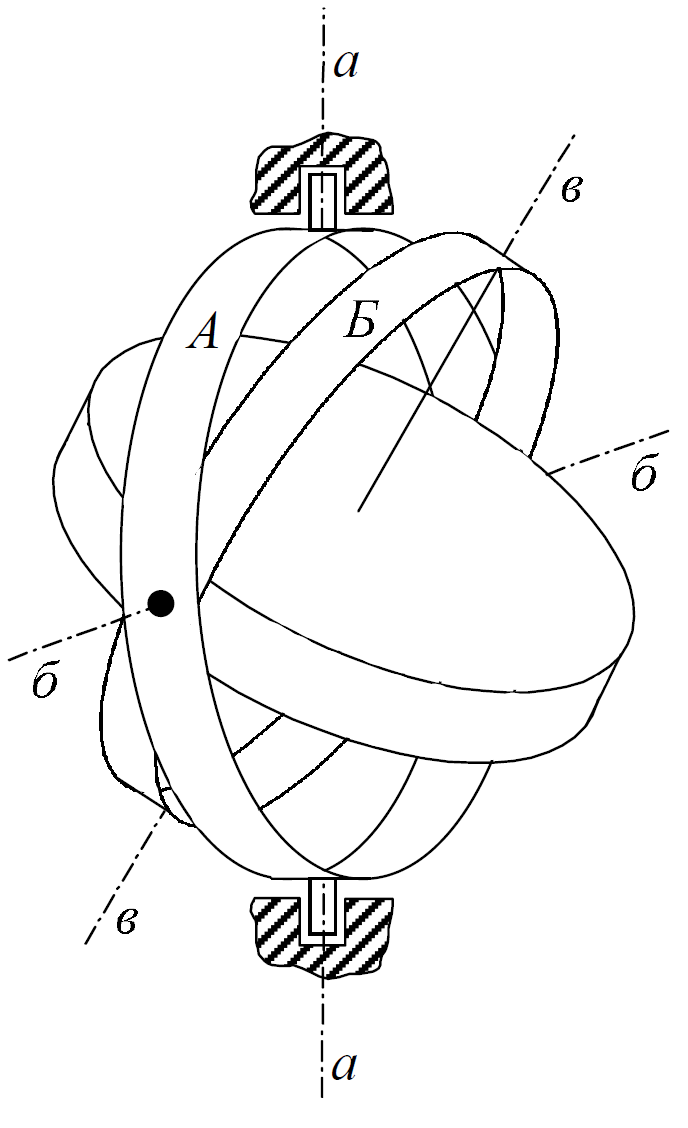
\includegraphics[width=0.3\textwidth]{giroscope.png}
	\caption{\textit{Гироскоп в кордановом подвесе}}
	\label{giroscope}
\end{figure}

Экспериментальная установка для исследования прецессии уравновешенного гироскопа показана на рис. \ref{ustan}. Ротором гироскопа является ротор высокооборотного электромотора М, питающегося током частотой 400 Гц. Кожух мотора (статор, имеющий обмотки, питаемые током частотой 400 Гц) скреплен с кольцом Б (рис. \ref{giroscope} и \ref{ustan}). Мотор с кольцом Б может вращаться в кольце А вокруг горизонтальной оси \textit{бб}, которое может вращаться вокруг вертикальной оси \textit{аа}. Ротор электромотора представляет массивный стальной цилиндр с прожилками меди, образующими «беличье колесо». Обозначенный на рис. \ref{ustan} буквой С рычаг направлен по оси симметрии ротора. На рычаг подвешивают грузы Г. Подвешивая различные грузы, можно менять силу F, момент которой определяется расстоянием 1 от точки подвеса до горизонтальной оси кольца А (до центра масс гироскопа), указанным на самой установке. 

Выше при выводе формул для прецессии предполагалось, что действующие на гироскоп силы лежат в плоскости $zy$, в которой лежат векторы угловых скоростей собственного вращения и прецессии. В этом случае, как уже говорилось, момент сил меняет лишь направление момента импульса гироскопа, но не его величину. Силы трения не лежат в плоскости осей вращения. Они приводят к изменению момента импульса и по направлению, и по величине. Для ротора гироскопа действие сил трения скомпенсировано действием электромотора. Для осей карданова подвеса компенсации нет. В результате ось гироскопа будет опускаться в направлении действия груза.

\begin{figure}[h!]
        \centering
	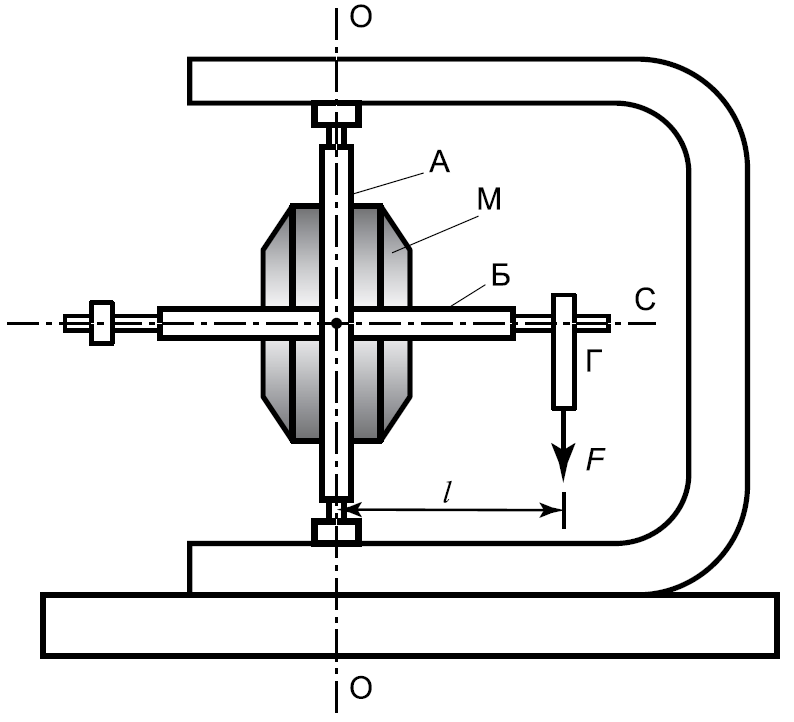
\includegraphics[width=0.6\textwidth]{ustan.png}
	\caption{\textit{Схема экспериментальной установки}}
	\label{ustan}
\end{figure}

Для исследвания зависимости скорости прецессии гироскопа от момента силы к оси гироскопа (к рычагу С) подвешиваются грузы Г. Скорость прецессии определяется по числу оборотов рычага вокруг вертикальной оси и времени, которое на это ушло, определяемое секундомером. В процессе измерений рычаг поворачивается и опускается в результате прецессии гироскопа. Поэтому его следует приподнять на $\text{5-6}^\circ$. Опыт надо закончить, когда рычаг опустится на такой же угол.

Угловую скорость вращения ротора гироскопа можно вычислить, используя формулу \eqref{prec-speed}. Момент инерции относительно оси симметрии $I_0$ измеряется по крутильным колебаниям точной копии ротора подвешенной вдоль оси симметрии на жесткой проволоке. Период крутильных колебаний $T_0$ зависит от момента инерции $I_0$ и модуля кручения проволоки $f$:

\begin{equation}
    T_{0} = 2 \pi \sqrt{\frac{I_{0}}{f}}
\end{equation}

Для того, чтобы исключить модуль кручения проволоки можно подвесить цилиндр с известными размерами и массой, тогда момент инерции ротора гироскопа вычисляется как

\begin{equation}\label{rotor-inertia}
    I_{0} = I_{\text{ц}} \frac{T_{0}^2}{T_{\text{ц}}^2}
\end{equation}

где $T_{\text{ц}}$ -- период крутильных колебаний цилиндра.

Ротор электромотора всегда немного намагничен. При вращении он навоит во второй обмотке переменную ЭДС индукции, частота которой равна частоте вращения ротора. Частоту этой ЭДС можно измерить по фигурам Лиссажу, получаемым на экране осцилографа, если на один выход подать исследуемую ЭДС, а на другой -- переменное напряжение с генератора. Таким образом есть ещё один способ измерения скорости вращения ротора.

\section{Оборудование и экспериментальные погрешности}

\textbf{Секундомер:} $\sigma_s = \pm 0,6$ с \\ 
\textbf{Электронные весы ВЛТЭ-5100:} $\sigma_m = \pm 0,3$ г \\
\textbf{Штангенциркуль:} $\sigma_\text{шт} = \pm 0,005$ см \\

\section{Результаты измерений и обработка данных}
\subsection{Подготовка установки}

Установим ось гироскопа в горизонтальное положение, осторожно поворачивая её за рычаг $C$.

\subsection{Включение гироскопа}

Включим питание гироскопа. Подождём 5 минут, чтобы вращение ротора гироскопа успело стабилизироваться.

\subsection{Проверка гироскопа}

Убедимся в том, что скорость вращения ротора достаточно большая. Будем легко постукивать по рычагу $C$. Он не изменяет своего положения в пространстве. Гироскоп остаётся неподвижен, так как момент силы, возникающей при постукивании действует на протяжении малого промежутка времени и не успевает изменить положение гироскопа.

Понажимаем карандашом на рычаг $C$ под различными углами, в процессе возникает регулярная прецессия гироскопа, обусловленная моментом силы нажатия. При нажатии вниз, гироскоп вращается против часовой стрелки, значит ветор вращения ротора $\vec{\omega}$ напрвален из центра гироскопа по направлению к рычагу $C$.

\subsection{Подвешивание груза}

Подвесим к рычагу $C$ груз. При этом начинается прецессия гироскопа. Во время вращения возникает сила трения в вертикальной оси подвеса Кордана, противодействующая вращению. Под действием момента силы трения рычаг будет медленно опускаться.

\subsection{Измерение прецессии гироскопа}
\label{4-5}


Длина плеча указана на установке: $l = (121 \pm 0,1) \text{ мм}$

Сначала необходимо измерить массы грузов с помощью электронных весов. Запишем результаты измерений в таблицу \ref{mass}.

\begin{table}[!ht]
    \centering
    \begin{tabular}{|l|l|l|l|l|l|}
    \hline
        № груза & 1 & 2 & 3 & 4 & 5 \\ \hline
        масса, г, & 328,5 & 217,4 & 141,9 & 91,1 & 56,7 \\ \hline
        $\sigma_m$, г, & 0,1 & 0,1 & 0,1 & 0,1 & 0,1 \\ \hline
    \end{tabular}\caption{\textit{Массы грузов}}\label{mass}
\end{table}

Подвесим к гироскопу груз и с помощью секундомера найдем угловую скорость регулярной прецессии гироскопа. Отклоним рычаг на угол $5^\circ$ (погрешность измерения угла $\sigma_\varphi = 1,5^\circ$) вверх в вертикальной оси и измерим время, за которое он опустится, повтори этот опыт 3 раза для каждого груза и запишем в таблицу \ref{precession-1} сразу результаты для периодов прецессии.

\begin{table}[!ht]
    \centering
    \begin{tabular}{|l|l|l|l|l|l|l|}
    \hline
        № гр & № оп & t, c & $N_\text{об}$ & T, с & $\sigma_T, \text{ с}$ & $T_\text{ср}$ \\ \hline
        \multirow{3}{*}{1} & 1 & 123,95 & 4 & 30,99 & 0,2 & \multirow{3}{*}{31,0} \\ \cline{2-6}
        ~ & 2 & 123,88 & 4 & 30,97 & 0,2 & ~ \\ \cline{2-6}
        ~ & 3 & 124,73 & 4 & 31,18 & 0,2 & ~ \\ \hline
    \end{tabular}\caption{\textit{Измерение периода прецессии для груза 1}}\label{precession-1}
\end{table}

\subsection{Измерения прецессии для всех грузов}

Повторим серию экспериментов для из пункта \ref{4-5} и результаты запишем в таблицу \ref{precession}. Сразу найдём скорость прецесии и вычислим момент силы $M = mgl$.

% \begin{table}[!ht]
%     \centering
%     \begin{tabular}{|l|l|l|l|l|l|l|l|l|l|}
%     \hline
%         № гр & № оп & t, c & $N_\text{об}$ & T, с & $T_\text{ср}$ & $\Omega_\text{ср}$, $\text{ с}^{-1}$ & $M$, $\text{Н} \cdot \text{м}$ & $\sigma_\Omega$, $\text{ с}^{-1}$ & $\sigma_M$, $\text{Н} \cdot \text{м}$ \\ \hline
%         \multirow{3}{*}{1} & 1 & 123,95 & 4 & 30,99 & \multirow{3}{*}{31,0} & \multirow{3}{*}{0,202} & \multirow{3}{*}{0,3895} & \multirow{3}{*}{} & \multirow{3}{*}{0,0005} \\ \cline{2-5}
%         ~ & 2 & 123,88 & 4 & 30,97 & ~ & ~ & ~ & ~ & ~ \\ \cline{2-5}
%         ~ & 3 & 124,73 & 4 & 31,18 & ~ & ~ & ~ & ~ & ~ \\ \hline
%         \multirow{3}{*}{2} & 1 & 187,44 & 4 & 46,86 & \multirow{3}{*}{46,8} & \multirow{3}{*}{0,134} & \multirow{3}{*}{0,2578} & \multirow{3}{*}{} & \multirow{3}{*}{0,0004} \\ \cline{2-5}
%         ~ & 2 & 140,47 & 3 & 46,82 & ~ & ~ & ~ & ~ & ~ \\ \cline{2-5}
%         ~ & 3 & 187,39 & 4 & 46,85 & ~ & ~ & ~ & ~ & ~ \\ \hline
%         \multirow{3}{*}{3} & 1 & 288,00 & 4 & 72,00 & \multirow{3}{*}{73,1} & \multirow{3}{*}{0,086} & \multirow{3}{*}{0,1683} & \multirow{3}{*}{} & \multirow{3}{*}{0,0004} \\ \cline{2-5}
%         ~ & 2 & 225,50 & 3 & 75,17 & ~ & ~ & ~ & ~ & ~ \\ \cline{2-5}
%         ~ & 3 & 216,13 & 3 & 72,04 & ~ & ~ & ~ & ~ & ~ \\ \hline
%         \multirow{3}{*}{4} & 1 & 456,55 & 4 & 114,14 & \multirow{3}{*}{114,1} & \multirow{3}{*}{0,055} & \multirow{3}{*}{0,1080} & \multirow{3}{*}{} & \multirow{3}{*}{0,0004} \\ \cline{2-5}
%         ~ & 2 & 693,75 & 6 & 115,63 & ~ & ~ & ~ & ~ & ~ \\ \cline{2-5}
%         ~ & 3 & 337,47 & 3 & 112,49 & ~ & ~ & ~ & ~ & ~ \\ \hline
%         \multirow{3}{*}{5} & 1 & 360,48 & 2 & 180,24 & \multirow{3}{*}{180,5} & \multirow{3}{*}{0,035} & \multirow{3}{*}{0,0672} & \multirow{3}{*}{} & \multirow{3}{*}{0,0004} \\ \cline{2-5}
%         ~ & 2 & 361,02 & 2 & 180,51 & ~ & ~ & ~ & ~ & ~ \\ \cline{2-5}
%         ~ & 3 & 361,49 & 2 & 180,75 & ~ & ~ & ~ & ~ & ~ \\ \hline
%     \end{tabular}\caption{\textit{Измерение периодов прецессии гироскопа}}\label{precession}
% \end{table}


\begin{table}[!ht]
    \centering
    \begin{tabular}{|l|l|l|l|l|l|l|l|}
    \hline
        № гр & № оп & t, c & $N_\text{об}$ & T, с & $T_\text{ср}$ & $\Omega_\text{ср}$, $\text{ с}^{-1}$ & $M$, $\text{Н} \cdot \text{м}$ \\ \hline
        \multirow{3}{*}{1} & 1 & 123,95 & 4 & 30,99 & \multirow{3}{*}{31,0} & \multirow{3}{*}{0,202} & \multirow{3}{*}{0,3895} \\ \cline{2-5}
        ~ & 2 & 123,88 & 4 & 30,97 & ~ & ~ & ~ \\ \cline{2-5}
        ~ & 3 & 124,73 & 4 & 31,18 & ~ & ~ & ~ \\ \hline
        \multirow{3}{*}{2} & 1 & 187,44 & 4 & 46,86 & \multirow{3}{*}{46,8} & \multirow{3}{*}{0,134} & \multirow{3}{*}{0,2578} \\ \cline{2-5}
        ~ & 2 & 140,47 & 3 & 46,82 & ~ & ~ & ~ \\ \cline{2-5}
        ~ & 3 & 187,39 & 4 & 46,85 & ~ & ~ & ~ \\ \hline
        \multirow{3}{*}{3} & 1 & 288,00 & 4 & 72,00 & \multirow{3}{*}{73,1} & \multirow{3}{*}{0,086} & \multirow{3}{*}{0,1683} \\ \cline{2-5}
        ~ & 2 & 225,50 & 3 & 75,17 & ~ & ~ & ~ \\ \cline{2-5}
        ~ & 3 & 216,13 & 3 & 72,04 & ~ & ~ & ~ \\ \hline
        \multirow{3}{*}{4} & 1 & 456,55 & 4 & 114,14 & \multirow{3}{*}{114,1} & \multirow{3}{*}{0,055} & \multirow{3}{*}{0,1080} \\ \cline{2-5}
        ~ & 2 & 693,75 & 6 & 115,63 & ~ & ~ & ~ \\ \cline{2-5}
        ~ & 3 & 337,47 & 3 & 112,49 & ~ & ~ & ~ \\ \hline
        \multirow{3}{*}{5} & 1 & 360,48 & 2 & 180,24 & \multirow{3}{*}{180,5} & \multirow{3}{*}{0,035} & \multirow{3}{*}{0,0672} \\ \cline{2-5}
        ~ & 2 & 361,02 & 2 & 180,51 & ~ & ~ & ~ \\ \cline{2-5}
        ~ & 3 & 361,49 & 2 & 180,75 & ~ & ~ & ~ \\ \hline
    \end{tabular}\caption{\textit{Измерение периодов прецессии гироскопа}}\label{precession}
\end{table}

Построим график зависимости $\Omega$ от $M$. Воспользуемся МНК для аппроксимации наилучшей прямой. В данном случае $u = \Omega$, а $v = M$. Так как зависимость согласно формуле \eqref{prec-speed} должна быть линейной, получаем:

% Из формулы \eqref{prec-speed} следует, что зависимость скорости прецессии от момента силы -- линейная. Для проверки этой зависимости 

\begin{equation}
    k = \frac{\langle uv\rangle}{\langle v^2 \rangle} = 0,518 \ \frac{1}{\text{Н} \cdot \text{м} \cdot \text{с}}
\end{equation}

Найдём погрешность $\sigma_k$:

\begin{equation}
    \sigma_k = \frac{1}{\sqrt{5}} \sqrt{\frac{\langle u^2 \rangle}{\langle v^2 \rangle} - k^2} = 0,001 \ \frac{1}{\text{Н} \cdot \text{м} \cdot \text{с}}
\end{equation}

Нанесём прямую и экспериментальные точки на график, изображённый на рисунке \ref{omega-M}. Как видно из графика зависимость выполняется достаточно точно.

\subsection{Измерение момента инерции ротора}

Измерим момент инерции ротора гироскопа относительно оси симметрии $I_0$. Для этого подвесим ротор к концу вертикальной висящей проволоки так, чтобы ось симметрии ротора была вертикальна. Измерим период колебаний получившегося крутильного маятника для $n = 20$ колебаний:

\begin{equation}
    T_{n} = 63,3 \text{ с} \ \ \ \ T_0 = \frac{T_{n}}{n} = 3,17 \text{ с}
\end{equation}

Проведём аналогичные измерения для цилиндра диаметром $d = 7,8 \text{ см}$, массой $m_\text{ц} = 1616,6 \text{ г}$:

\begin{equation}
    T_{\text{ц}n} = 80,2 \text{ с} \ \ \ \ T_\text{ц} = \frac{T_{\text{ц}n}}{n} = 4,01 \text{ с}
\end{equation}

Погрешность вычисления времени для одного периода вычисляется как: $\sigma_T = \frac{\sigma_s}{n} = 0,03 \text{ с}$

Момент инерции цилиндра можно вычислить по формуле:

\begin{equation}
    I_\text{ц} = \frac{m d^2}{8} = 1,229 \text{ г} \cdot \text{м}^2
\end{equation}

Подставим это в формулу \eqref{rotor-inertia}:

\begin{equation}
    I_{0} = \frac{m d^2 T_{0}^2}{8T_{\text{ц}}^2} = 0,77 \text{ г} \cdot \text{м}^2
\end{equation}

\subsection{Оценка погрешностей}

Рассчитаем погрешности измерения регулярной прецесии гироскопа для каждой серии опытов и запишем их в таблицу \ref{precession-error}. Систематическа погрешность измерения прецесии для каждого измерения вычисляется по формуле: $\sigma_\Omega^\text{сист} = \frac{\sigma_T}{T} \cdot \Omega$. Случайная погрешность вычисляется по формуле: \\ $ \sigma_{\Omega}^\text{случ} = \sqrt{\frac{1}{N  (N-1)}\sum(\Omega_i-\overline{\Omega})^2}$

Погрешность для момента инерции ротора можно рассчитать по формуле:

\begin{equation}
    \sigma_{I_0} = \sqrt{
    \left( \frac{dI_0}{dm} \right) ^ 2 \sigma_{m}^2 + 
    \left( \frac{dI_0}{dd} \right) ^ 2 \sigma_{d}^2 + 
    \left( \frac{dI_0}{dT_0} \right) ^ 2 \sigma_{T_0}^2 + 
    \left( \frac{dI_0}{dT_{\text{ц}}} \right) ^ 2 \sigma_{T_{\text{ц}}}^2
    } \approx 0,02 \text{ г} \cdot \text{м}^2
\end{equation}

\subsection{Рассчёт частоты вращения ротора}

Согласно формуле \eqref{prec-speed} зависимость $\Omega$ от $M$ имеет вид:

\begin{equation}
    \Omega = \frac{M}{I_0 \omega_0}
\end{equation}

А так же нам изветно значение $k = 0,518 \ \frac{1}{\text{Н} \cdot \text{м} \cdot \text{с}}$, при этом:

\begin{equation}
    \Omega = k M
\end{equation}

Откуда следует, что:

\begin{equation}
    k = \frac{1}{I_0 \omega_0} \ \ \ \implies \ \ \omega_0 = \frac{1}{I_0 k} \implies \nu = \frac{1}{2 \pi I_0 k} = 400 \text{ Гц}
\end{equation}

Погрешность частоты вращения можно вычислить по формуле:

\begin{equation}
    \sigma_\nu = \nu \sqrt{ \left (\frac{\sigma_k}{k} \right)^2 + 
    \left (\frac{\sigma_{I_0}}{I_0}\right)^2 } = 10 \text{ Гц}
\end{equation}

В итоге получаем, что частота вращения ротора равна: $\nu = ( 400 \pm 10 ) \text{ Гц}$. А так же $\omega_0 = 2 \pi \nu = ( 2520 \pm 60 ) \text{ с}^{-1}$

\subsection{Определение момента сил трения}

Так как угол отклонения рычага мал, то $\Omega_\text{тр} = 2 \varphi \Omega$. Так же получаем:

\begin{equation}
    m g l = \Omega L \ \ \ \text{и} \ \ \ M_\text{тр} = \Omega_\text{тр} L
\end{equation}

Откуда следует, что:

\begin{equation}
    M_\text{тр} = mgl \frac{\Omega_\text{тр}}{\Omega} = 2 m g l \varphi
\end{equation}

Погрешность для моментов сил трения вычисляется по формуле:

\begin{equation}
    \sigma_{M_\text{тр}} = M_\text{тр} \sqrt{
    \left ( \frac{\sigma_{m}}{m} \right)^2 +
    \left ( \frac{\sigma_{l}}{l} \right)^2 +
    \left ( \frac{\sigma_{\varphi}}{\varphi} \right)^2
    }
\end{equation}

Подсчитаем моенты сил трения, их погрешность и запишем в таблицу \ref{friction}.

\begin{table}[!ht]
    \centering
    \begin{tabular}{|l|l|l|l|l|}
    \hline
        m, г & $\varphi$ & $M_\text{тр}$ & $\sigma_{M_\text{тр}}$ & $\varepsilon$, $\%$ \\ \hline
        328,5 & 10 & 0,068 & 0,010 & 15\% \\ \hline
        217,4 & 10 & 0,045 & 0,007 & 15\% \\ \hline
        141,9 & 10 & 0,029 & 0,004 & 15\% \\ \hline
        91,1 & 10 & 0,019 & 0,003 & 15\% \\ \hline
        56,7 & 10 & 0,012 & 0,002 & 15\% \\ \hline
    \end{tabular}\caption{\textit{Вычисление моментов сил трения}}\label{friction}
\end{table}

\subsection{Определение частоты вращения ротора по фигурам Лиссажу}

Подадим на «Вход Y» осциллографа сигнал со второй обмотки статора гироскопа, а на «Вход синхр.» сигнал с выхода генератора. Теперь получим на экране осцилографа фигуру Лиссажу. Добъёмся того, чтобы фигура была похожа на эллипс. После этого подберём такую частоту генератора, чтобы фигура была неподвижна. Такая частота будет являтся частотой вращения ротора гироскопа: $\nu = (376,3 \pm 0,3 ) \text{ Гц}$.

\subsection{Сравнение полученных значений}

Полученные значения для частоты вращения ротора не совпадают в пределах в погрешности, но при этом имеют одинаковый порядок.

\subsection{Применимость соотношения \eqref{condition-9}}

Моменты инерции практически не отличаются в разных осях. При этом имеем $\frac{\Omega}{\omega_0} \ll 1$. откуда получаем $\frac{L_\Omega}{L_{\omega_0}} \ll 1 \implies L_\Omega \ll L_{\omega_0}$, что и является соотношением \eqref{condition-9}.

\section{Обсуждение результатов и выводы}

В ходе работы была исследована прецессия гироскопа и получены значения её скорости для различных воздействий на гироскоп.

Было установлено, что зависимость скорости вынужденной прецессии от величины момента сил является линейной.

Была определена скорость и частота вращения ротора гироскопа двумя различными способами. Эти значения были сравнены друг с другом.

\begin{figure}[h]
    \begin{center}$
        \begin{array}{cc}
            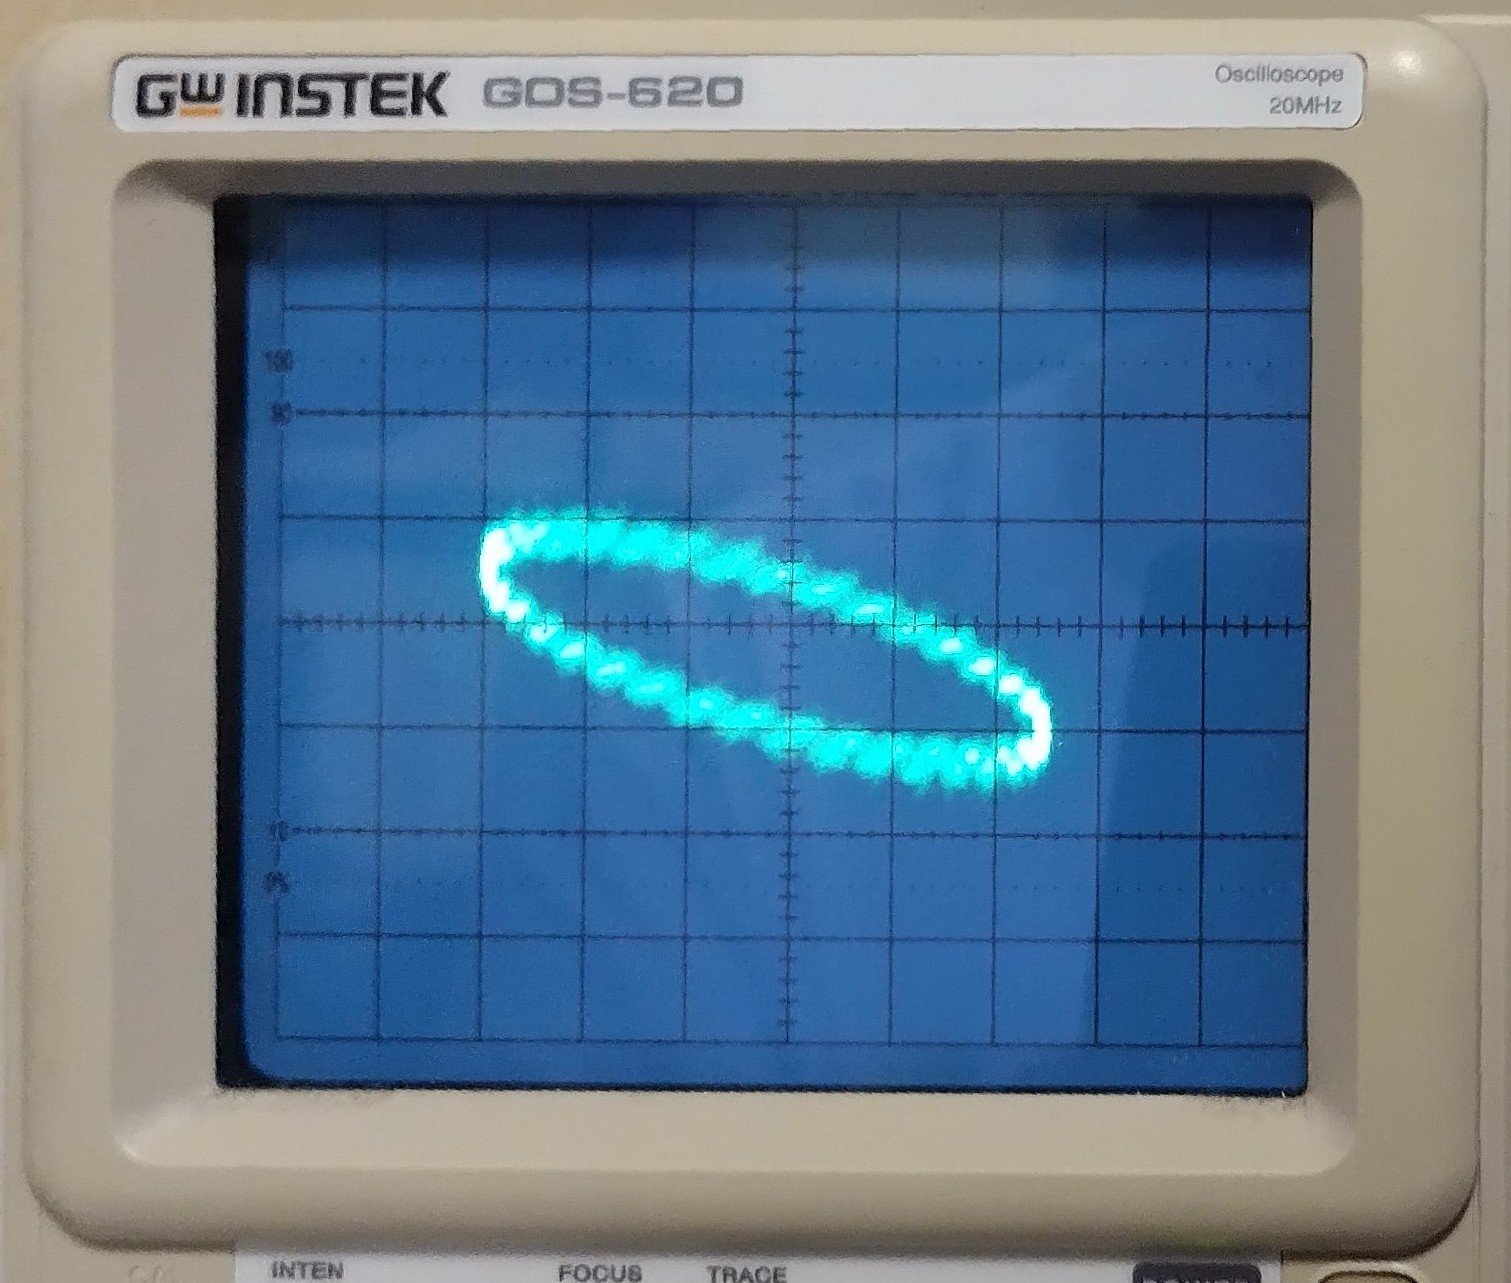
\includegraphics[width=0.45\textwidth]{oscilator.jpg}&
            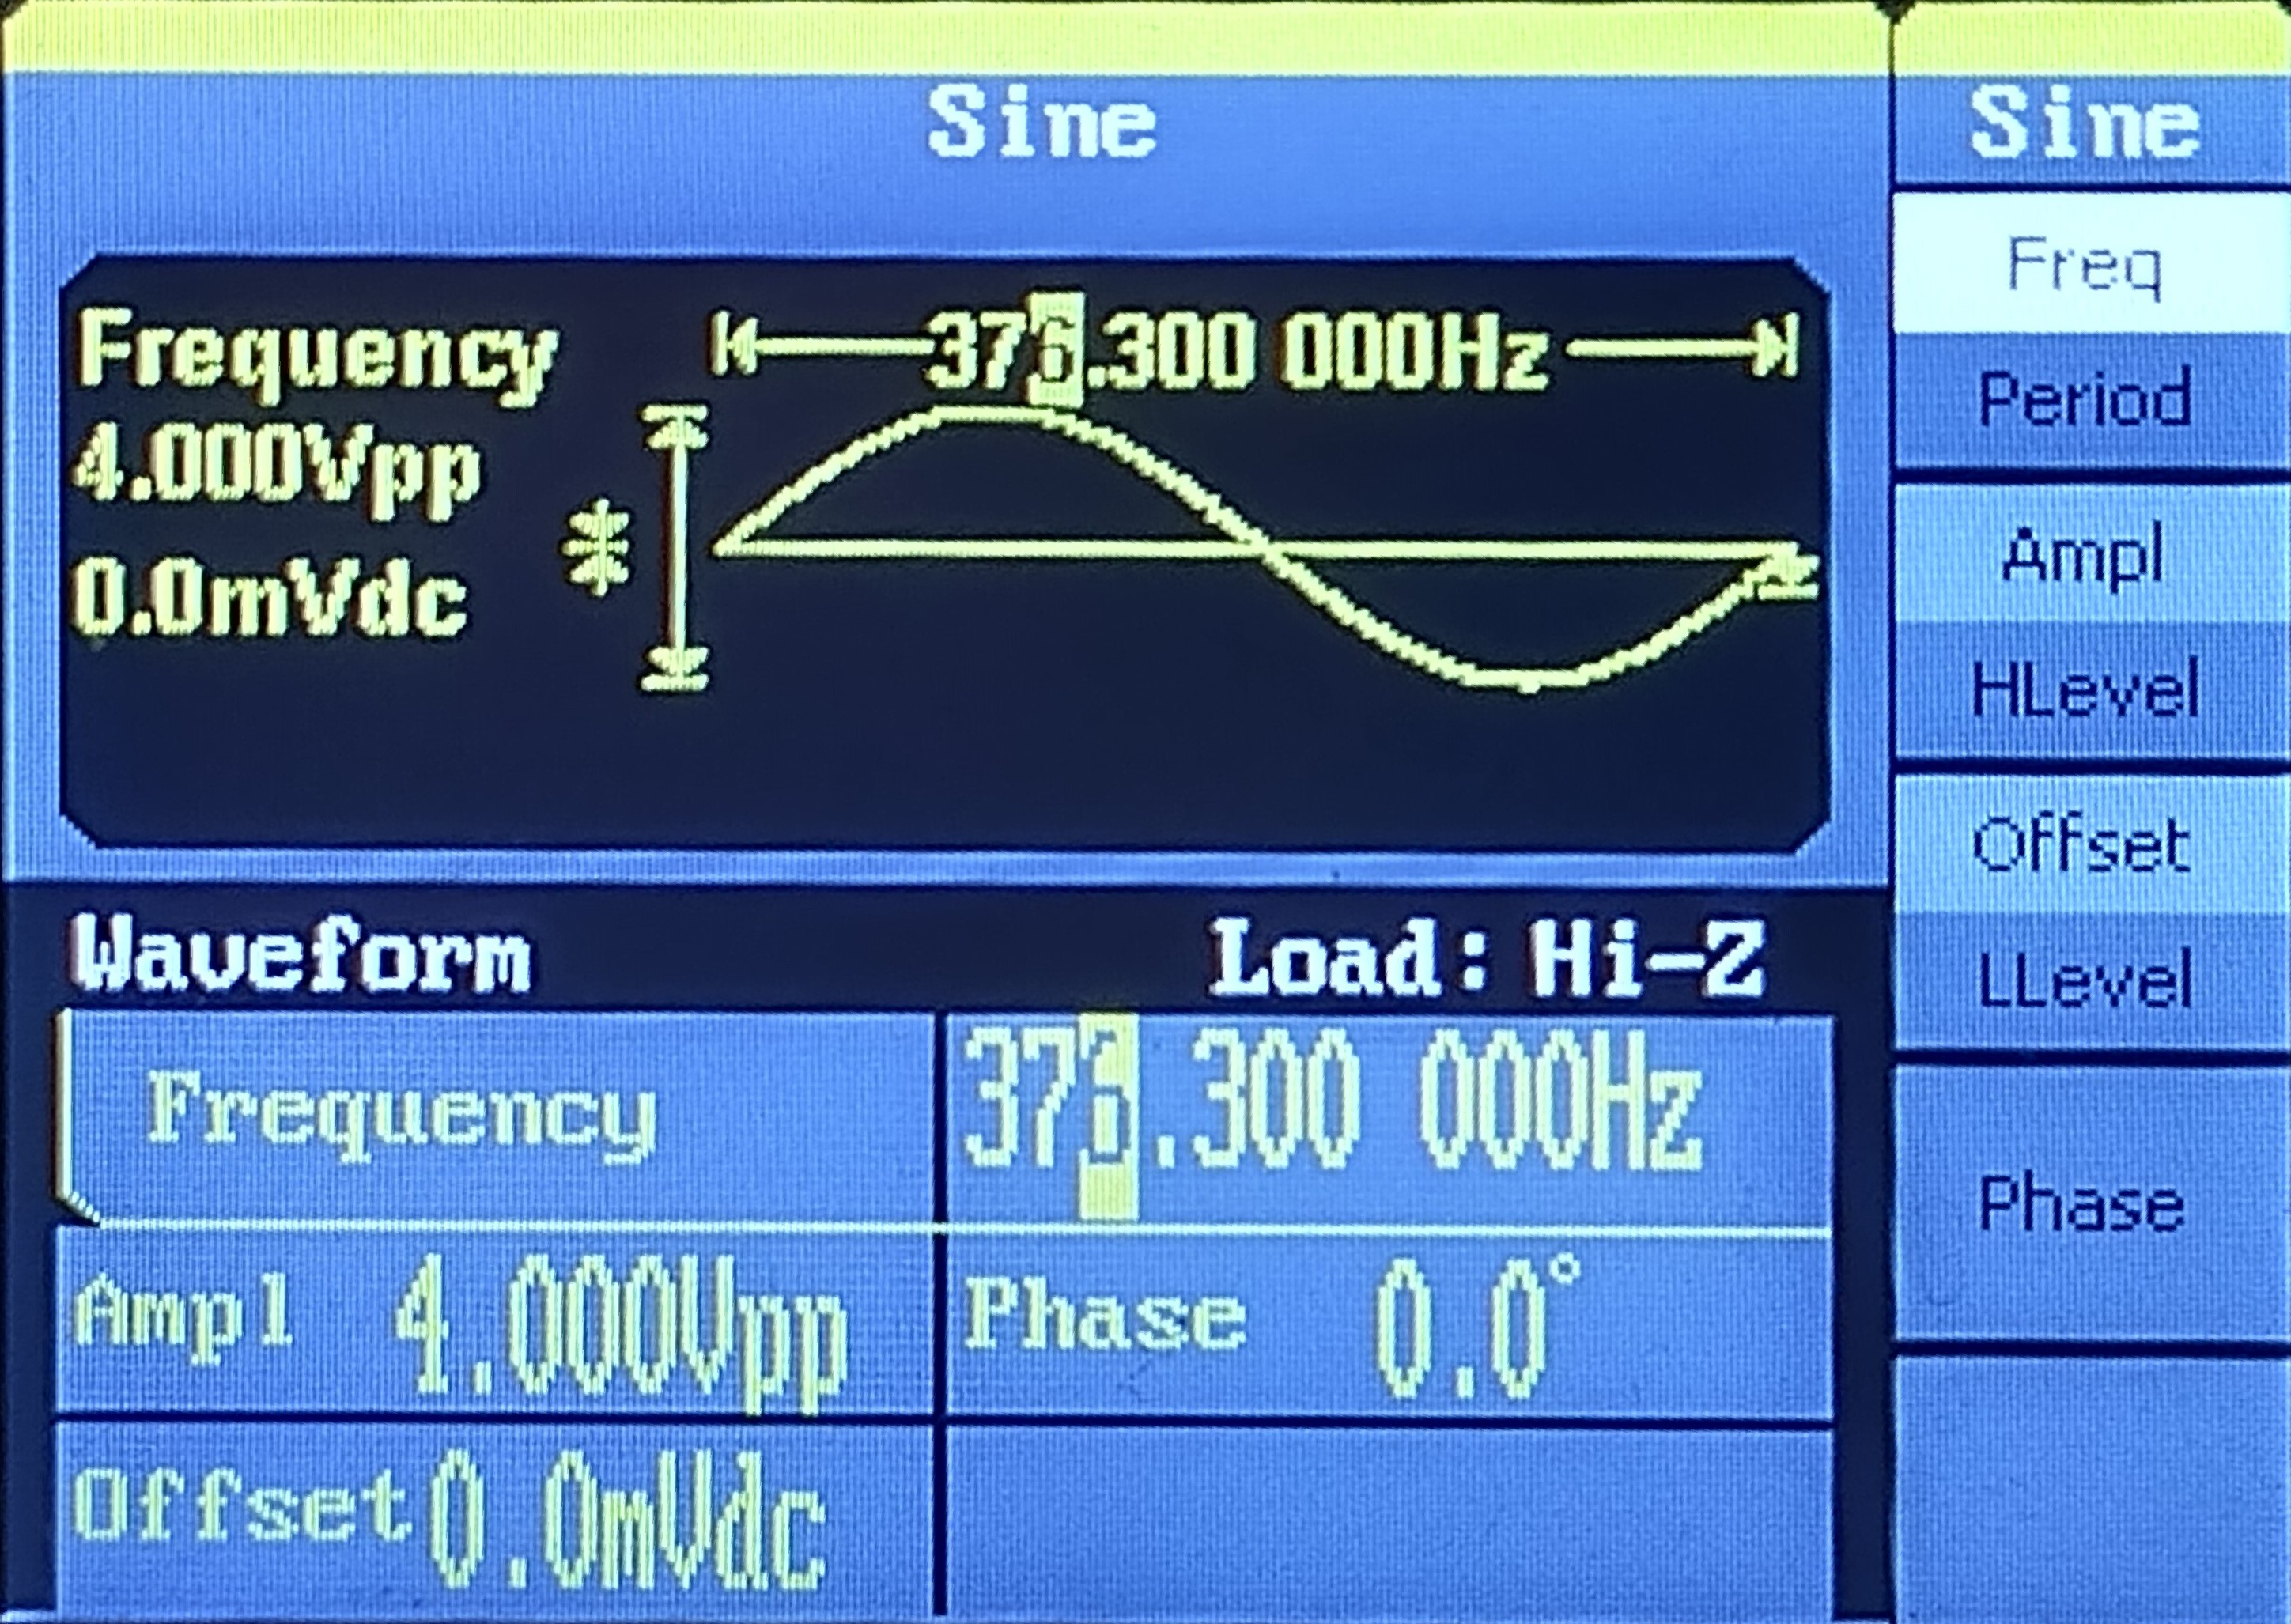
\includegraphics[width=0.45\textwidth]{generator.jpg}\\
        \end{array}$
    \end{center}
    \caption{Полученная фигура Лиссажу и частота генератора}
    \label{fig:ustan1}
\end{figure}


\begin{table}[!h]
    \centering
    \begin{tabular}{|l|l|l|l|l|l|l|l|l|l|l|}
    \hline
        № гр & № & t, c & $N_\text{об}$ & T, с & $\Omega$, $\text{ с}^{-1}$ & $\sigma_\Omega^\text{сист}$, $\text{ с}^{-1}$ & $\sigma_\Omega^\text{сист}$, $\text{ с}^{-1}$ & $\sigma_\Omega^\text{случ}$, $\text{ с}^{-1}$ & $\sigma_\text{полн}$, $\text{ с}^{-1}$ & $\varepsilon$, $\%$ \\ \hline
        \multirow{3}{*}{1} & 1 & 123,95 & 4 & 30,99 & 0,203 & 0,00131 & \multirow{3}{*}{0,00130} & \multirow{3}{*}{0,00044} & \multirow{3}{*}{0,00138} & \multirow{3}{*}{0,7} \\ \cline{2-7}
        ~ & 2 & 123,88 & 4 & 30,97 & 0,203 & 0,00131 & ~ & ~ & ~ & ~ \\ \cline{2-7}
        ~ & 3 & 124,73 & 4 & 31,18 & 0,201 & 0,00129 & ~ & ~ & ~ & ~ \\ \hline
        \multirow{3}{*}{2} & 1 & 187,44 & 4 & 46,86 & 0,134 & 0,00057 & \multirow{3}{*}{0,00057} & \multirow{3}{*}{0,00003} & \multirow{3}{*}{0,00057} & \multirow{3}{*}{0,4} \\ \cline{2-7}
        ~ & 2 & 140,47 & 3 & 46,82 & 0,134 & 0,00057 & ~ & ~ & ~ & ~ \\ \cline{2-7}
        ~ & 3 & 187,39 & 4 & 46,85 & 0,134 & 0,00057 & ~ & ~ & ~ & ~ \\ \hline
        \multirow{3}{*}{3} & 1 & 288,00 & 4 & 72,00 & 0,087 & 0,00024 & \multirow{3}{*}{0,00024} & \multirow{3}{*}{0,00122} & \multirow{3}{*}{0,00124} & \multirow{3}{*}{1,4} \\ \cline{2-7}
        ~ & 2 & 225,50 & 3 & 75,17 & 0,084 & 0,00022 & ~ & ~ & ~ & ~ \\ \cline{2-7}
        ~ & 3 & 216,13 & 3 & 72,04 & 0,087 & 0,00024 & ~ & ~ & ~ & ~ \\ \hline
        \multirow{3}{*}{4} & 1 & 456,55 & 4 & 114,14 & 0,055 & 0,00010 & \multirow{3}{*}{0,00010} & \multirow{3}{*}{0,00044} & \multirow{3}{*}{0,00045} & \multirow{3}{*}{0,8} \\ \cline{2-7}
        ~ & 2 & 693,75 & 6 & 115,63 & 0,054 & 0,00009 & ~ & ~ & ~ & ~ \\ \cline{2-7}
        ~ & 3 & 337,47 & 3 & 112,49 & 0,056 & 0,00010 & ~ & ~ & ~ & ~ \\ \hline
        \multirow{3}{*}{5} & 1 & 360,48 & 2 & 180,24 & 0,035 & 0,00004 & \multirow{3}{*}{0,00004} & \multirow{3}{*}{0,00002} & \multirow{3}{*}{0,00004} & \multirow{3}{*}{0,1} \\ \cline{2-7}
        ~ & 2 & 361,02 & 2 & 180,51 & 0,035 & 0,00004 & ~ & ~ & ~ & ~ \\ \cline{2-7}
        ~ & 3 & 361,49 & 2 & 180,75 & 0,035 & 0,00004 & ~ & ~ & ~ & ~ \\ \hline
    \end{tabular}\caption{\textit{Оценка погрешностей измерения прецесии гироскопа}}\label{precession-error}
\end{table}

\begin{figure}[h!]
    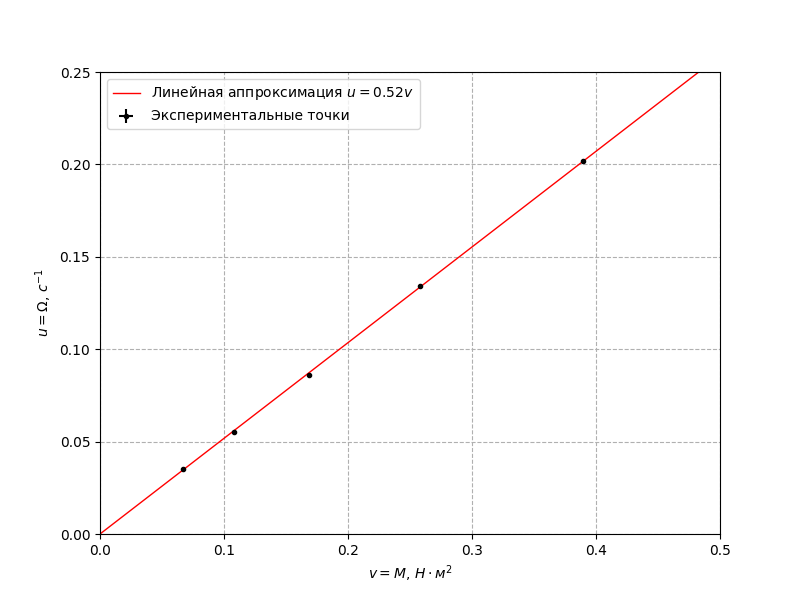
\includegraphics[width=1\textwidth]{graph.png}
    \caption{\textit{График зависимости $\Omega$ от $M$}}
    \label{omega-M}
\end{figure}


\end{document}